\clearpage
\begin{savequote}[8cm]
\textlatin{Neque porro quisquam est qui dolorem ipsum quia dolor sit amet, consectetur, adipisci velit...}

There is no one who loves pain itself, who seeks after it and wants to have it, simply because it is pain...
  \qauthor{--- Cicero's \textit{de Finibus Bonorum et Malorum}}
\end{savequote}

\chapter{\label{ch:8-systematics}Systematics} 

\minitoc

\section{Systematics}
\label{sec:systematics}

In this section, various sources of systematic uncertainty that affect the measurement are investigated. Many fixed parameters are used in the fit model and each need to be assigned a systematic uncertainty. Systematics are computed either by multiple fits to data with certain parameters smeared or in a toy setup where the generation is different to the fit model. 

\subsection{Sources of systematic uncertainty}

The branching ratios, MC efficiencies, PID efficiencies, veto efficiencies, and production, detection and PID asymmetries all have associated systematic uncertainties. These are estimated by performing multiple fits to data where the relevant fixed parameter are varied according to a Gaussian whose width is the assigned uncertainty. For each fit observable a histogram is created containing the results for each data fit, the RMS of this histogram is taken to be the systematic uncertainty for this parameter.

Signal shape, partially reconstructed contribution, combinatoric shape and charmless contribution all all have associated systematic uncertainties. These are computed using a toy setup where the generated model is different to the fit model. The systematic is taken to be the difference between the mean of the fitted distribution and the generated value.

\subsubsection{Branching ratios}

The branching ratios for the different \D decays are used in the \CP fit as shown in Equation \ref{effcorrectionglw}. The values used for the branching ratios are given in Table \ref{fitinputs} along with their uncertainties~\cite{PDG2014}. A systematic is assigned by performing 1000 fits to data each time varying the branching ratio values by a Gaussian with a width corresponding to the uncertainty of each branching ratio.

\subsubsection{MC efficiencies}

Selection efficincies and BDT efficiencies are used in the \CP fit as shown in Equations \ref{effcorrectionglw} and \ref{effcorrectionads}. The values used in the \CP fit are shown in Table \ref{fitinputs} along with their uncertainties. These values are fixed in the \CP fit. The Run 2 uncertainties are estimated assuming 2016 MC efficiencies have the same central value as 2015 but with twice the uncertainty.  A systematic is assigned by performing 1000 fits to data each time varying these fixed parameters according to a Gaussian whose width is the assigned unceratinty for that parameter.

\subsubsection{PID efficiencies}

PID efficiencies are used in the \CP fit as shown in Equation \ref{effcorrectionglw} and the values used are shown in Table \ref{fitinputs}. A systematic is assigned by performing 1000 fits to data each time varying the PID efficiencies according to a Gaussian whose width is the assigned unceratinty for that value.

\subsubsection{Veto efficiencies}

Veto efficiencies are required in the \CP fit to correct for the veto applied in the ADS mode, as shown in Equation \ref{effcorrectionads}, with the actual values used shown in Tables \ref{fitinputs} as well as the uncertainties. The Run 2 uncertainties are estimated assuming 2016 MC efficiencies have the same central value as 2015 but with twice the uncertainty. A systematic is assigned by performing 1000 fits to data each time varying the veto efficiencies according to a Gaussian whose width is the assigned unceratinty for that value.

\subsubsection{Asymmetry corrections}

Corrections must be made in the \CP for various sources of asymmetry as detailed in Section \ref{sec:cpfit:asymmetries}, namely production asymmetry, detection asymmetry and PID asymmetry. For each source of asymmetry a correction is applied in the \CP fit and a systematic is assigned separately to each based on the uncertainty of each correction. Details of the values used with their corresponding uncertainties are given in Section \ref{sec:cpfit:asymmetries}. It is worth noting that for production asymmetry, the Run 2 value is taken to have the same central value as Run 1 with double the uncertainty. 

\subsubsection{Signal shape}
\label{sec:systematics:signal}

The signal shape, described in Section \ref{sec:massfit:signal}, is modelled as a Double Crystal Ball with all the parameters fixed from MC apart from the mean and width. From signal MC it can be seen that the signal shape has more than one characteristic width a low mass tail. There are two sources of unceratinty in the choice of signal shape: the tail parameters, $\alpha$ and $n$, and the width ratio and yield fraction, $f_{\sigma}$ and $f_{cb}$, between the two CBs. These two sources of uncertainty are treated separately and combined. The uncertainty in the tail parameters is quantified by generating 1000 toys with a Double Johnson signal shape, but fitting back with the original fit model. The Double Johnson is taken to have the same width ratio and yield fraction as the Double Crystal Ball used in the \CP fit. The results from this method are given in the first row of Table \ref{signalshapeSystematics}.

For the uncertainty in the width ratio and yield fraction, a systematic is assigned by performing 1000 fits to data each time varying the width ratio and yield fraction according to a Gaussian whose width is the assigned unceratinty for that value, which is taken from the fits to MC, as given in Table \ref{signalparameters}. The results from this method are given in the second row of Table \ref{signalshapeSystematics}.

The systematic from generating a Double Johnson distribution and that from varying the Doule Crystal Ball parameters are added in quadrature to give the total signal shape systematic.

\begin{table}[h]
\centering
{\footnotesize
\begin{tabular}{ccccccccc}
\hline
& $A_{K\pi}$ & $A_{KK}$ & $A_{\pi\pi}$ & $R_{KK}$ & $R_{\pi\pi}$ & $R^+_{K\pi}$ & $R^-_{K\pi}$ \\
\hline
Johnson & $1.1 \times 10^{-3}$ & $2.9 \times 10^{-3}$ & $1.1 \times 10^{-2}$ & $3.0 \times 10^{-3}$ & $2.6 \times 10^{-2}$ & $1.0 \times 10^{-3}$ & $1.3 \times 10^{-3}$ \\
Vary params & $2.3 \times 10^{-4}$ & $1.1 \times 10^{-3}$ & $1.4 \times 10^{-3}$ & $5.9 \times 10^{-4}$ & $4.4 \times 10^{-3}$ & $2.2 \times 10^{-4}$ & $1.1 \times 10^{-4}$ \\
\hline
Total & $1.1 \times 10^{-3}$ & $3.1 \times 10^{-3}$ & $1.1 \times 10^{-2}$ & $3.0 \times 10^{-2}$ & $2.7 \times 10^{-2}$ & $1.1 \times 10^{-3}$ & $1.3 \times 10^{-3}$ \\
\hline
\end{tabular}
\begin{tabular}{cccccc}
\hline
& $A_{K\pi\pi\pi}$ & $A_{\pi\pi\pi\pi}$ & $R_{\pi\pi\pi\pi}$ & $R^+_{K3\pi}$ & $R^-_{K3\pi}$ \\
\hline
Johnson & $1.6 \times 10^{-3}$ & $1.3 \times 10^{-3}$ & $9.8 \times 10^{-3}$ & $3.0 \times 10^{-3}$ & $3.8 \times 10^{-3}$ \\
Vary params & $4.7 \times 10^{-4}$ & $1.8 \times 10^{-3}$ & $2.5 \times 10^{-3}$ & $2.4 \times 10^{-4}$ & $1.2 \times 10^{-4}$ \\
\hline
Total & $1.7 \times 10^{-3}$ & $2.2 \times 10^{-3}$ & $1.0 \times 10^{-2}$ & $3.0 \times 10^{-3}$ & $3.8 \times 10^{-3}$ \\
\hline
\end{tabular}}
\caption{Summary of systematic uncertainties associated with the signal shape}
\label{signalshapeSystematics}
\end{table}

\subsubsection{Combinatoric}

The shape of the combinatoric is fixed across all \D modes, the statistics are not enough to have the shapes floating. In order to get an idea of the variation in combinatoric shape between different \D modes, fits are performed to the high B mass region (5400 - 5600 \mevcc) using an exponential as the fit model, as shown in Figures \ref{combinatoricLL} and \ref{combinatoricDD}. The data used for these fits is Run 1 data with stripping and pre-selection applied, except for \Kstar selection and \Dz and \KS FD significance cuts. PID selection on the \D daughters is also applied in order to be sure of accessing the difference between the different \D modes. The full selection was not applied as there is not enough statistics to perform a meaningful fit.

\begin{figure}[h]
\centering
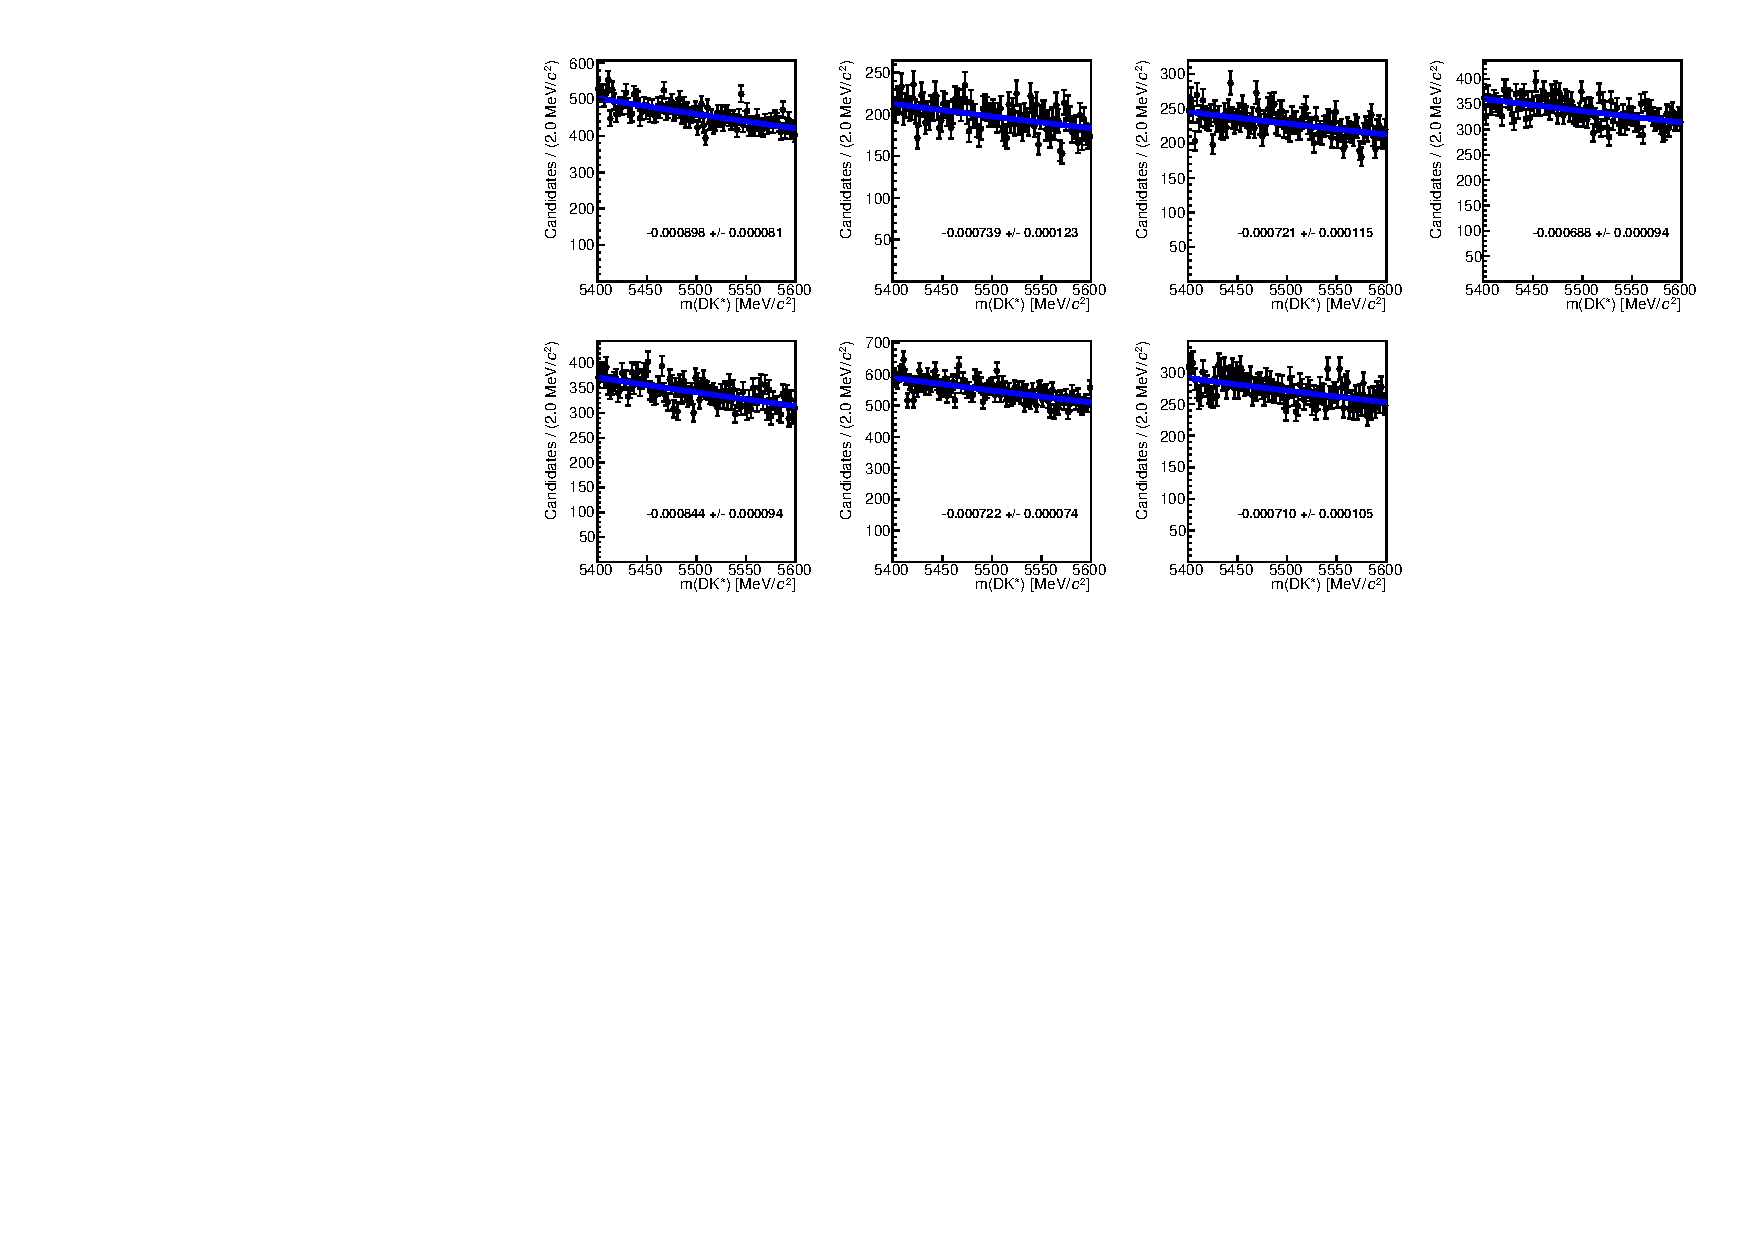
\includegraphics[width=\linewidth]{figures/fitComponents/combinatoricFits_LL.pdf}
\caption{Fits to the combinatoric background in the high B mass region for LL candidates. The fitted values for the exponential slope parameter are given on each plot}
\label{combinatoricLL}
\end{figure}

\begin{figure}[h]
\centering
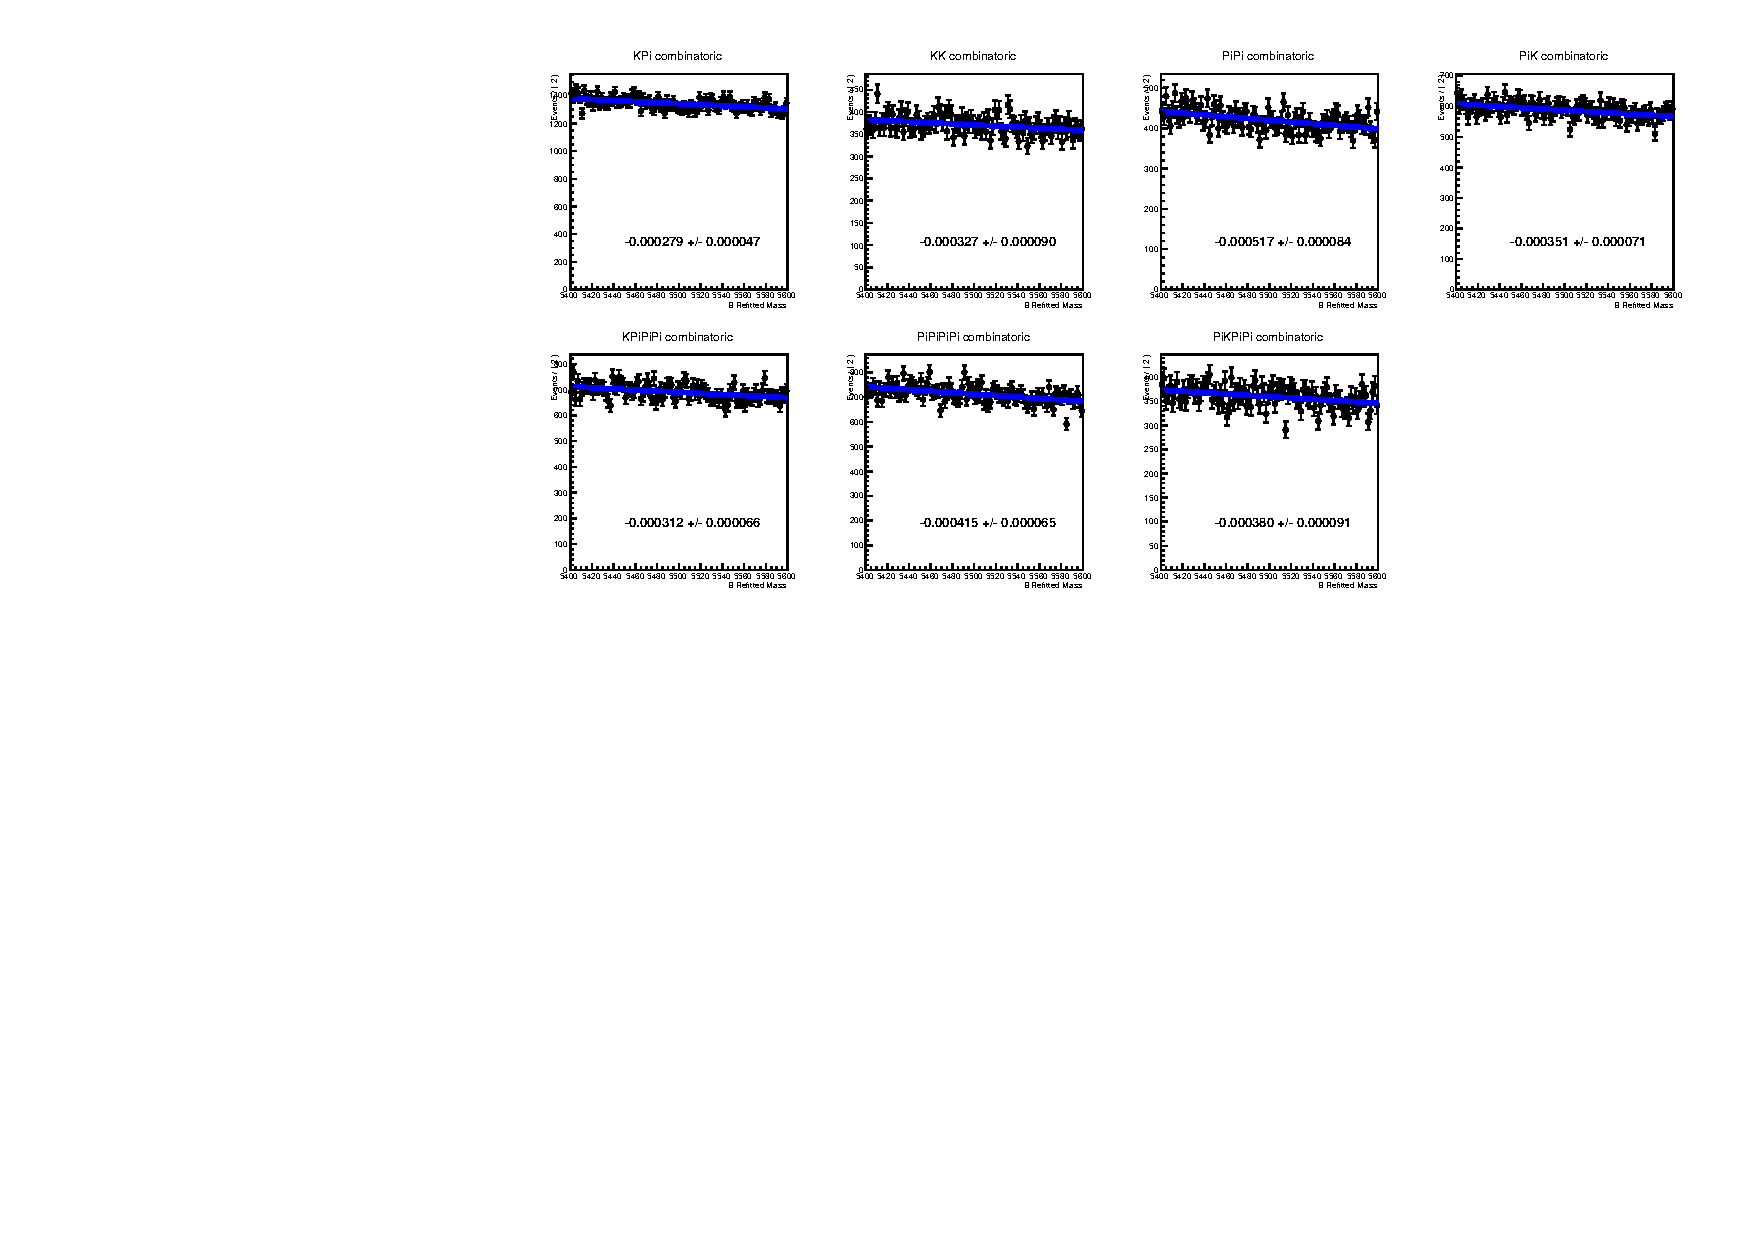
\includegraphics[width=\linewidth]{figures/fitComponents/combinatoricFits_DD.pdf}
\caption{Fits to the combinatoric background in the high B mass region for DD candidates. The fitted values for the exponential slope parameter are given on each plot}
\label{combinatoricDD}
\end{figure}

The systematic is assigned by generating 1000 toys with the combinatoric shape parameter for each mode fixed to those given in Figures \ref{combinatoricLL} and \ref{combinatoricDD}, but fitting back with the original fit model.

\subsubsection{Partially reconstructed}
\label{sec:systematics:partreco}

The partially reconstructed decays have a completely fixed shape and yield contributing to the \CP fit. The shape parameters are fixed from fits to MC, yield ratios are fixed from branching ratios and MC efficiencies and total yield is fixed from the fit to $K\pi$ invariant mass. The estimated yield is divided equally between \Bp and \Bm bins. In order to assign a systematic three different modifications are made to the partially reconstructed region:

\begin{itemize}
\item The yield is incrased by 20\%. The uncertainty in the yield from the fit to $K\pi$ invariant mass is about 5\%, but this is considered to be an underestimate, therefore a conservative systematic of 20\% is used
\item All partially reconstructed shape are smeared by the difference in signal width between MC and data. The width for all partially reconstructed shapes is increased by 4\% of LL bins and 5\% for DD bins
\item A 10\% asymmetry is introduced for the partially reconstructed shapes
\end{itemize}

These adjustments are applied simultaneously. The systematic is assigned by generating 1000 toys with the above modifications implemented, but fitting back with the original fit model.

\subsubsection{Charmless}

Section \ref{sec:backgrounds:charmless} shows that there is a possibility for residual charmless contribution in \decay{\D}{\pi\pi} mode. Charmless events in the $\pi\pi$ mode were generated according to a Gaussian whose mean is the expected number of charmless events and the width is the corresponding unceratinty, as given in Tables \ref{charmlessyields} and \ref{charmlessyieldsRun2}. This value is rounded to a whole number and randomly distributed between \Bp and \Bm as a component of the yield in the signal region. The systematic is assigned by generating 1000 toys with a charmless contrbution introduced, but fitting back with the original fit model.

\subsection{Results}

Table \ref{systematics} summarises the systematics for various different sources. If the systematic unceratinty was found to be more than 2 orders of magntiude smaller than the statistical unceratinty then a value of zero is given. Systematics from MC efficiencies and branching ratios mainly affects $R_{KK}$ and $R_{\pi\pi}$. Production and detection asymmetry systematics contribute to $A_{K\pi}$, $A_{KK}$ and $A_{\pi\pi}$. PID efficiencies and PID asymmetry correction do not contribute much to the systematic uncertainty. The signal shape systematic have a non-negligible effect on the uncertainty for all the physics observables. All systematic uncertainties are smaller than the corresponding statistical uncertainty. 

\begin{sidewaystable}
\centering
{\footnotesize
\begin{tabular}{ccccccccccccc}
\hline
& $A_{K\pi}$ & $A_{KK}$ & $A_{\pi\pi}$ & $R_{KK}$ & $R_{\pi\pi}$ & $R^+_{K\pi}$ & $R^-_{K\pi}$ & $A_{K\pi\pi\pi}$ & $A_{\pi\pi\pi\pi}$ & $R_{\pi\pi\pi\pi}$ & $R^+_{K3\pi}$ & $R^-_{K3\pi}$ \\
\hline
Statistical & $0.023$ & $0.07$ & $0.13$ & $0.09$ & $0.15$ & $0.006$ & $0.004$ & $0.031$ & $0.11$ & $0.13$ & $0.008$ & $0.007$ \\
\hline
BRs  & $0.0$ & $0.0$ & $0.013$ & $0.001$ & $0.012$ & $0.0$ & $0.0$ & $0.0$ & $0.0008$ & $0.027$ & $0.0$ & $0.0$ \\
MC efficiencies  & $0.0$ & $0.0$ & $0.007$ & $0.0$ & $0.006$ & $0.0002$ & $0.0$ & $0.0$ & $0.0005$ & $0.010$ & $0.0$ & $0.0$ \\
PID efficiencies  & $0.0$ & $0.0$ & $0.002$ & $0.0$ & $0.002$ & $0.0$ & $0.0$ & $0.0$ & $0.0$ & $0.003$ & $0.0$ & $0.0$ \\
Veto efficiencies  & $0.0$ & $0.0$ & $0.0$ & $0.0$ & $0.0$ & $0.0001$ & $0.0$ & $0.0$ & $0.0$ & $0.0$ & $0.0$ & $0.0$ \\
$A_{prod}$  & $0.0073$ & $0.007$ & $0.0$ & $0.008$ & $0.0$ & $0.0$ & $0.0$ & $0.0079$ & $0.0077$ & $0.0$ & $0.0$ & $0.0$ \\
$A_{det}$  & $0.0034$ & $0.003$ & $0.0$ & $0.003$ & $0.0$ & $0.0001$ & $0.0$ & $0.0034$ & $0.0030$ & $0.0$ & $0.0001$ & $0.0$ \\
$A_{pid}$ & $0.0$ & $0.0$ & $0.0$ & $0.0$ & $0.0$ & $0.0$ & $0.0$ & $0.0$ & $0.0$ & $0.0$ & $0.0$ & $0.0$ \\
Signal shape & $0.0011$ & $0.003$ & $0.011$ & $0.030$ & $0.027$ & $0.0011$ & $0.0013$ & $0.0017$ & $0.0022$ & $0.010$ & $0.0030$ & $0.0038$ \\
Combinatoric shape  & $0.0012$ & $0.003$ & $0.004$ & $0.005$ & $0.009$ & $0.0002$ & $0.0003$ & $0.0001$ & $0.0018$ & $0.0$ & $0.0012$ & $0.0004$ \\
Partially reconstructed shape  & $0.0007$ & $0.001$ & $0.001$ & $0.003$ & $0.005$ & $0.0$ & $0.0003$ & $0.0003$ & $0.0005$ & $0.002$ & $0.0008$ & $0.0001$ \\
Charmless  & $0.0008$ & $0.0$ & $0.002$ & $0.003$ & $0.007$ & $0.0$ & $0.0003$ & $0.0009$ & $0.0030$ & $0.002$ & $0.0008$ & $0.0001$ \\
\hline
Total & $0.0083$ & $0.009$ & $0.019$ & $0.012$ & $0.032$ & $0.0011$ & $0.0014$ & $0.0088$ & $0.0093$ & $0.031$ & $0.0034$ & $0.0038$ \\
\hline
\end{tabular}}
\caption{Summary of systematic uncertainties}
\label{systematics}
\end{sidewaystable}


\clearpage
